% !Mode:: "TeX:UTF-8"
\graphicspath{{chapter/}{figures/}}
%%%%%%%%%%%%%%%%%%%%%%%%%%%%%%
%% 封面部分
%%%%%%%%%%%%%%%%%%%%%%%%%%%%%%
\begin{titlepage}
	\centering
	
\includegraphics[width=0.2\textwidth]{sf1.png}\par
	\vspace{1cm}
	
\includegraphics[width=0.8\textwidth]{sf.jpg}\par
	\vspace{0.1cm}
	{\scshape\LARGE Harbin Institute of Technology \par}
	\vspace{1cm}
	{\kaishu\LARGE 开关电源设计开发实践与创新思维课程报告\par}
	\vspace{1.5cm}
	{\huge\bfseries 交错串联电容分接Buck降压电路ISC-TaB\par}
	\vspace{2cm}
	{\fangsong\Large\itshape 蒋佳诚\par}
	\vfill
	{1180610825}\par
	\fangsong{电气工程及自动化系}
	\vfill
	指导教师	\textsc{管乐诗}
	\vfill
% Bottom of the page
	{\large \today\par}
\end{titlepage}

\chapter{研究背景及意义}
高降压比DC/DC变换器在工业、汽车、电信领域得到广泛应用。随着数据中心和云计算的不断发展,对电能传输的效率等指标提出了更高要求。在数据中心领域,流行的降压比为60V/48V/24V到5V/3.3V/1.8V。


Buck电路是一种典型的DC/DC拓扑结构。Buck电路结构简单,实现成本低,在电力电子与工业领域应用广泛。但是,对于一个二级Buck电路,要提高降压比,需要MOS管承受窄导通时间带来的大电流,这就在材料上对功率开关提出了极高要求。同时,高降压比所需要的极低占空比需要更高效的PWM,实际实施困难。这些因素限制了二级Buck电路的应用。


串联电容Buck电路(Series-capacitor Buck,SC-Buck)把开关电容和多相Buck结合到一起,形成一种新的Buck电路的拓扑结构。与传统的Buck电路相比,SC-Buck规模更小,效率更高,具有电流自平衡功能。如图1-1所示,两个电感交错放置于电路中,消除输出电容$C_o$上的电流纹波,同时还能分别减小两个电感的尺寸。图1-2表明,分到每条支路上的电压只有输入电压的一半。


实现高降压比的另一个趋势是使用磁性元件。实现方法有带倍流整流的全桥变换器(full-bridge converter with current-doubler rectifier),LLC,Sigma变换器和分接电感Buck变换器(tapped inductor Buck converter)等。在轻载时,全桥变换器无法实现所有主开关管的零电压开关(Zero-voltage Switching),导致轻载时转换效率下降,而且输出端的大电感会影响功率密度。在谐振频率下,LLC具有较高效率,但是系统不在谐振频率时的动态效率很低。为了解决这个问题,提出了将LLC和Buck结合的Sigma变换器。LLC负责谐振频率下的高效功率传输,Buck变换器负责瞬态响应。但是,由于LLC变换器在稳态时处理大部分的功率,Buck变换器在过渡时处理大部分的功率,因此LLC变换器和Buck变换器都必须设计成能够处理整个系统的功率。如此的并行结构将增大控制的复杂度。


Tapped inductor Buck转换器最初用于处理高降压比功率转换电路。然而,交错电感的漏感与开关电容产生共振,产生额外的电压环。基于混合变压器的Buck变换器(Hybrid-transformer-based Buck,HTB)增加了一个开关(S3)和一个电感,以获得软开关操作和较低的电压环,如图1-3所示。利用交错电感的漏感作为谐振电感,交错串联电容Buck(Series-capacitor tapped Buck,SC-TaB)变换器如图1-4所示。SC-TaB中的开关管$S_3$可以直接连接负载,也可以直接接地,另一种SC-TaB电路如图1-5所示。后者的两相交错配置的电路图如图1-6所示。开关管接地可以让控制更为简单。


SC-TaB和2ph-SC的主要优点是实现了所有开关管的ZVS,提高了转换效率。然而,随着降压比的增大,耦合电感的匝数比也随之增大,高匝数比会给耦合电感带来更多的应力,影响转换效率。为了克服这一缺点,并考虑到SC-Buck具有倍增降压比的能力,通过引入电容$C_1$,提出了一种新的变换器拓扑,如图1-7所示。新拓扑结构被称为交错串联电容分接Buck变换器(ISC-TaB)。该转换器将SC-Buck和SC-TaB的优点结合到一起。与传统的SC-TaB相比,它的降压比提高了一倍,使得该变换器更适合用于高降压比场合。
\begin{figure}[h]
    \centering
    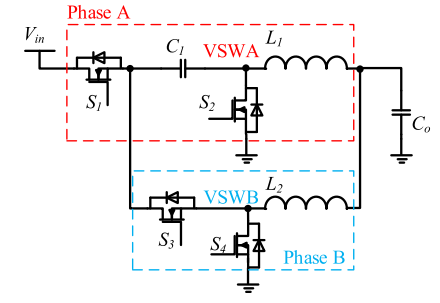
\includegraphics[width = 0.8\textwidth]{figures/SC-Buck.png}
    \caption{SC-Buck}
\end{figure}
\begin{figure}[h]
    \centering
    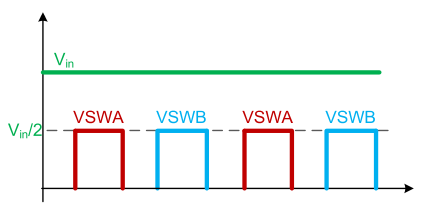
\includegraphics[width = 0.8\textwidth]{figures/SC-Buck_v.png}
    \caption{SC-Buck波形图}
\end{figure}
\begin{figure}[h]
    \centering
    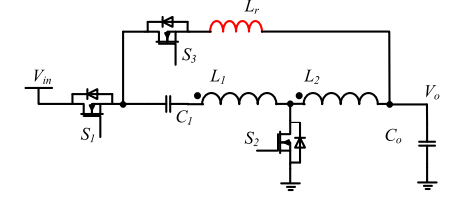
\includegraphics[width = 0.8\textwidth]{figures/HTB-Buck.png}
    \caption{HTB-Buck}
\end{figure}
\begin{figure}[h]
    \centering
    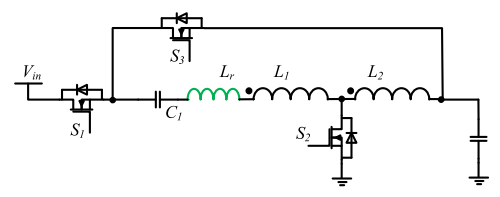
\includegraphics[width = 0.8\textwidth]{figures/SC-TaB1.png}
    \caption{SC-TaB,$S_3$接入负载}
\end{figure}
\begin{figure}[h]
    \centering
    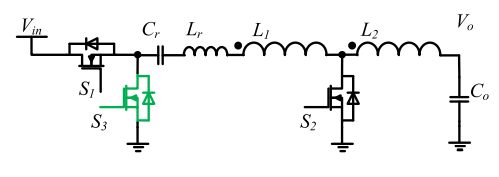
\includegraphics[width = 0.8\textwidth]{figures/SC-TaB.png}
    \caption{SC-TaB,$S_3$接地}
\end{figure}
\begin{figure}[h]
    \centering
    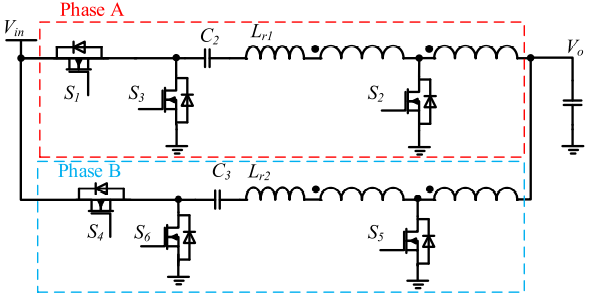
\includegraphics[width = 0.8\textwidth]{figures/2ph SC-TaB.png}
    \caption{2ph SC-TaB}
\end{figure}
\begin{figure}[h]
    \centering
    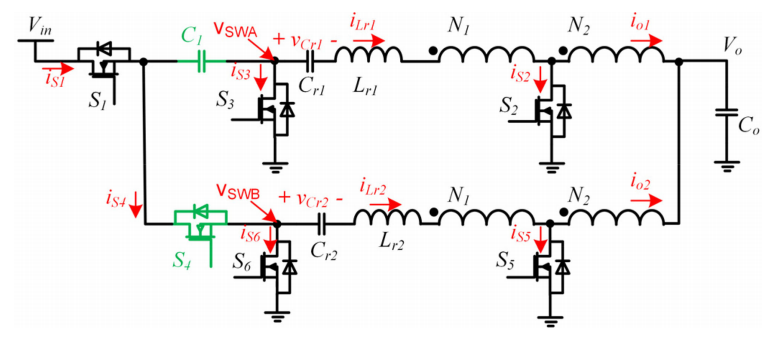
\includegraphics[width = 0.8\textwidth]{figures/circuit diagram1.png}
    \caption{ISC-TaB}
\end{figure}
\chapter{电路分析}
\section{电路结构}
\begin{figure}[h]
    \centering
    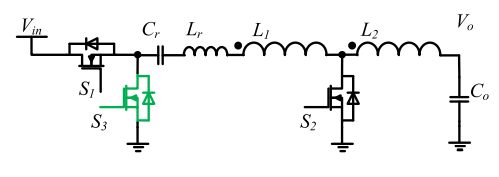
\includegraphics[width = 0.8\textwidth]{figures/SC-TaB.png}
    \caption{SC-TaB}
\end{figure}
\begin{figure}[h]
    \centering
    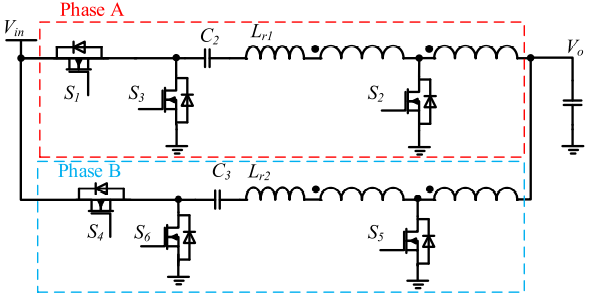
\includegraphics[width = 0.8\textwidth]{figures/2ph SC-TaB.png}
    \caption{2ph SC-TaB}
\end{figure}
\begin{figure}[h]
    \centering
    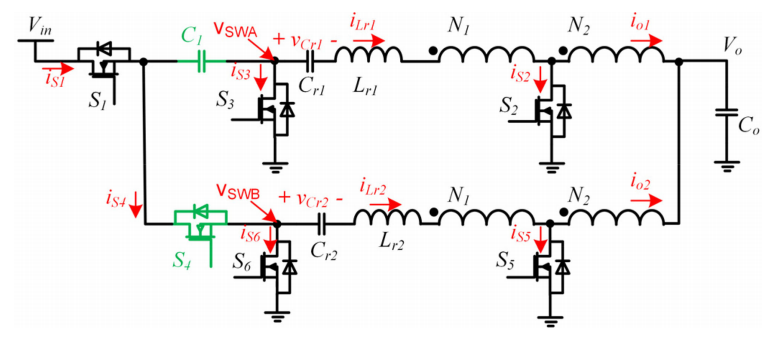
\includegraphics[width = 0.8\textwidth]{figures/circuit diagram1.png}
    \caption{ISC-TaB}
\end{figure}
\begin{figure}[h]
    \centering
    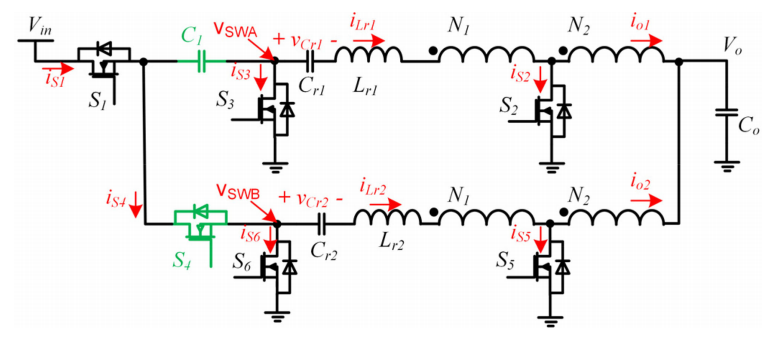
\includegraphics[width = 0.8\textwidth]{figures/circuit diagram1.png}
    \caption{ISC-TaB}
\end{figure}
电路采用了六个开关管,电容$C_1$将电路的两相分离。
\section{电路参数}
记小球直径为D,1号球由$h-2/d$高度处释放,则高度差为h。由动能定理,
\begin{equation}
	\frac{1}{2}  m_{1} v_{1}^{2} - 0 = m_{1 }g h
\end{equation}
\par
质量相等的两球发生对心正碰,有
\begin{equation}
	m_{1} = m_{2}
\end{equation}
\begin{equation}
	m_{1} v_{1} = m_{2} v_{2}
\end{equation}
\par
2号球做平抛运动,其距地高度为$H$,平抛距离为$R$,有
\begin{equation}
	H = \frac{1}{2} g t^{2}
\end{equation}
\begin{equation}
	R_{theory} = v_{2} t
\end{equation}
\par 
联立以上方程,解得$R-h$关系
\begin{equation}
	R_{theory} (h) = 2 \sqrt{Hh}
\end{equation}
\par
实验测得2号球距地高度$15.6cm$,代入得到一个一次函数关系
\begin{equation}
	R_{theory} (h) = 2 \sqrt{15.6 h}
\end{equation}

\subsection{实验值}
在实验中,对h每隔1cm进行5次重复实验,并取平均值得到$R_{average}$。同时假设发生对心正碰后的小球1静止,由2.1.1得到$v_{1}$,$v_{2}$:
\begin{equation}
	v_{1} = \sqrt{2gh}
\end{equation}
\begin{equation}
	v_{2} = R \sqrt{\frac{g}{2H}}
\end{equation}

分别求同一$h$处的$v_{1}$,$v_{2}$,并将其平均值记录到下表中。取$g = 9.8 m/s^{2}$


\begin{longtable}{ccccc}%
	\caption{\wuhao 实验数据处理}\\[0.3em]
	\toprule[1.5pt] 下落高度h(cm) & $R_{average}$(cm) & $R_{theory}(cm) $ & $v_{1,average}$(m/s) & $v_{2,average}$ (m/s) \\ \midrule[1pt]
	\endfirsthead
	\multicolumn{3}{r}{表~\thetable(续表)}\vspace{0.5em}\\
	\toprule[1.5pt] 下落高度h(cm) & $R_{average}$(cm) & $R_{theory}(cm) $ & $v_{1,average}$(m/s) & $v_{2,average}$ (m/s) \\ \midrule[1pt]
	\endhead
	\bottomrule[1.5pt]
	\endfoot
    3.00  & 12.90  & 13.68  & 0.77  & 0.72  \\
    4.00  & 13.96  & 15.80  & 0.89  & 0.78  \\
    5.00  & 15.48  & 17.66  & 0.99  & 0.87  \\
    6.00  & 17.26  & 19.35  & 1.08  & 0.97  \\
    7.00  & 18.88  & 20.90  & 1.17  & 1.06  \\
    8.00  & 20.48  & 22.34  & 1.25  & 1.15  \\
    9.00  & 21.50  & 23.70  & 1.33  & 1.20  \\
    10.00  & 24.28  & 24.98  & 1.40  & 1.36  \\
    11.00  & 25.66  & 26.20  & 1.47  & 1.44  \\
    12.00  & 26.70  & 27.36  & 1.53  & 1.50  \\
    13.00  & 27.98  & 28.48  & 1.60  & 1.57  \\
    14.00  & 28.10  & 29.56  & 1.66  & 1.57  \\
\end{longtable}\normalsize

\par
给出拟合曲线图:
\begin{figure}[h]
    \centering
    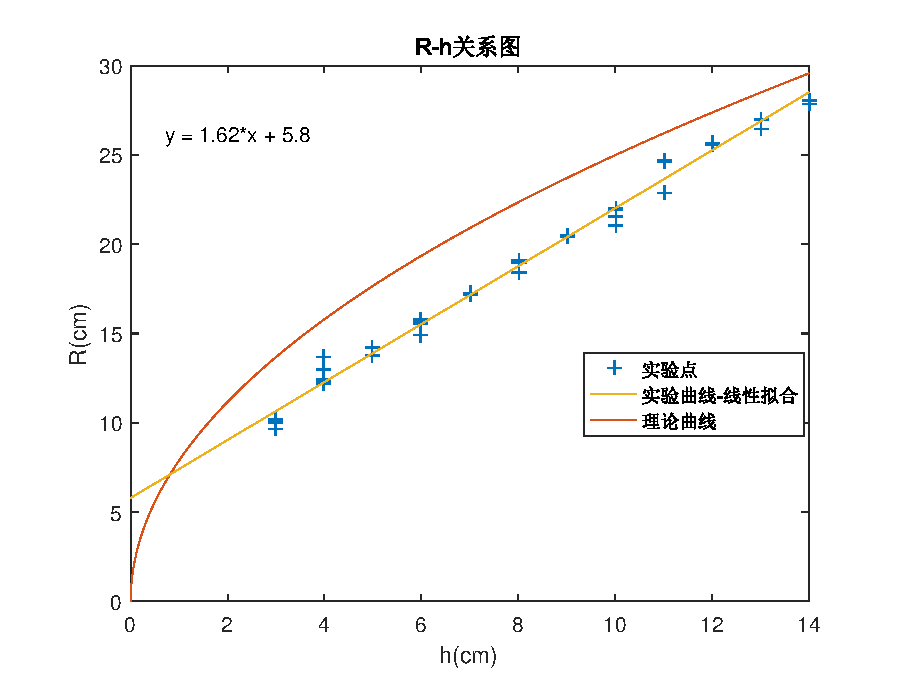
\includegraphics[width = 0.8\textwidth]{01}
    \caption{实验曲线与理论曲线}
\end{figure}

实验值拟合曲线为
\begin{equation}
	R_{Experiment} (h) = 1.62 h + 5.80
\end{equation}

可见,$R = 16.00$时,$h = 6.29$;
$R = 22.00$时,$h = 10.00$


\subsection{恢复系数}

假设碰撞后小球1无动能,则碰撞前速度差即为$v_{1}$,,碰撞后速度差即为$v_{2}$。由最小二乘法公式
\begin{equation}
	c=\frac{\overline{v_{1}v_{2}}-\bar{v_{1}}  \bar{v_{2}}}{\overline{v_{1}^{2}}-(\bar{v_{1}})^{2}}
\end{equation}

得到 $c = 0.98$
\begin{figure}[h]
    \centering
    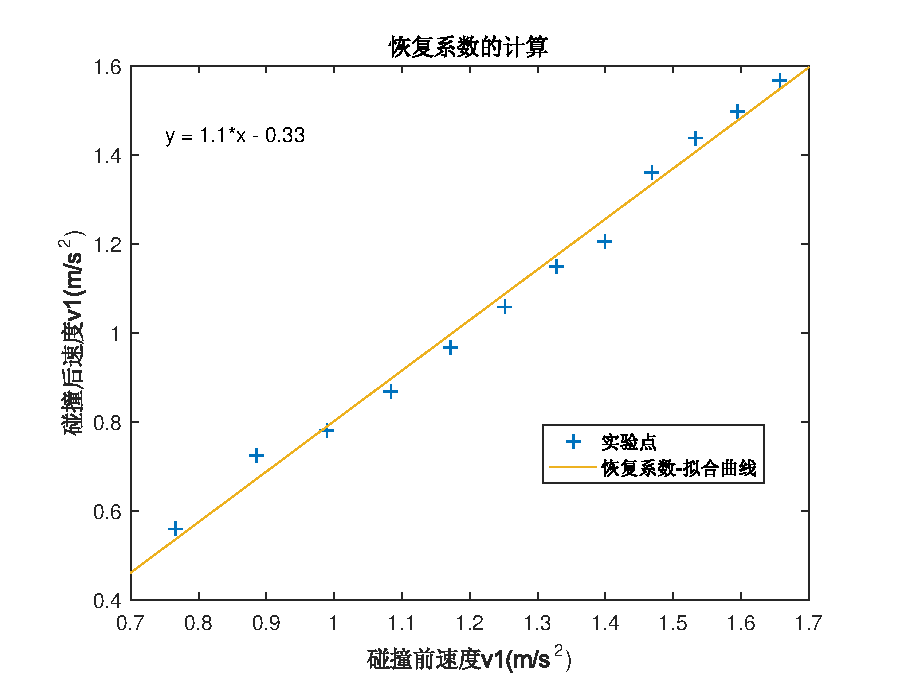
\includegraphics[width = 0.8\textwidth]{02}
    \caption{恢复系数}
\end{figure}

\chapter{仿真电路波形}
\section{$h$误差产生原因}
	装置摆放不水平,摆绳与球连接处的弯角附加的距离,人估读误差等。

\section{传递能量比与质量比之间的关系}
	由定义,传递能量比为:
\begin{equation}
	\epsilon = \frac{e}{E}\\
			 = \frac{\frac{1}{2}m_{2} v_{2}^{2}}{\frac{1}{2}m_{1} v_{1}^{2}} 
\end{equation}

\begin{equation}
	\epsilon = \frac{1}{\mu} \frac{v_{2}^{2}}{v_{1}^{2}} 
\end{equation}

\chapter{研究总结及思考}

\end{document}

